% Chapter 4

\chapter{Trying to improve the State of the Art}

\lhead{Chapter 5. \emph{Trying to improve the State of the Art}} % This is for the header on each page - perhaps a shortened title
\label{chp:refwork}
%----------------------------------------------------------------------------------------

\def\:{\hskip0pt} %Definisce un modo veloce per permettere a latex di sillabare correttamente anche parole come 4-connectivity. Il corretto utilizzo è il seguente: 4\:-\:connectivity.
The architeture proposed by Cipriano et al. was quite simple yet effective. The
main novel addition was the use of a positional encoding. We now want to try to
improve the results obtained by them by adding some more complex
and more recent architectures, losses and optimizers.

\section{Boundary Loss}
Jointly with PosPadUNet3D, standard DICE loss was used. We also tried to use
CrossEntropy loss, but the results were not as good as with DICE loss so it has
been discarded. As we were dealing with higly unbalanced data, less than 1\% of
the whole volume is the canal, we looked for alternative losses which deal with
this problem.

Kervadec et al. proposed a loss function which takes the form of a distance
metric on the space of contours instead of regions. Dice or cross-entropy, are
based on regional integrals, which are convenient for training deep neural
networks. In practice, these regional integrals are summations over the
segmentation regions of differentiable functions, each directly invoking the
softmax probability outputs of the network. Therefore, standard stochastic
optimizers such as SGD are directly applicable. Unfortunately, difficulties
occur for highly unbalanced segmentations, for instance, when the size of target
foreground region is several orders of magnitude less than the background size,
which is a common charactiristic for medical images. The problem of such losses
is that thet assumes identical importance distribution for all the samples and
classes.

In the proposed paper, the authors proposed a new type of loss, named
\emph{Boundary loss} that aims to mitigate the issues related to regional losses
in highly unbalanced segmentation problems. Rather than using unbalanced
integrals over the regions, a boundary loss uses integrals over the boundary
between the regions. Furthermore, it provides information that is complementary
to regional losses. It is, however, challenging to represent the boundary points
corresponding to the regional softmax outputs of a CNN. This difficulty may
explain why boundary losses have been avoided in the context of deep
segmentation networks.

\subsection{Formulation}
The Boundary loss has been formulated as follows:
let $I: \Omega \subset \mathbb{R}^{2,3} \rightarrow \mathbb{R}$ denotes an image
with spatial domain $\Omega$, and $g: \Omega \rightarrow {0,1}$ a binary ground
thruth segmentation of the image such that $g(p) = 1$ if the pixel $p$ belongs
to the target region $G \subset \Omega$ and $0$ otherwise. Let $s_\theta :
\Omega \rightarrow [0,1]$ denotes the softmax probability output of a deep
segmentation network, and $S_\theta \subset \Omega$ denotes the corresponding
segmentation region: $\S_\theta = {p \in \Omega | s_\theta(p) >= \delta}$ for
some threshold $\delta$. Let $\Delta G$ denote a representation of the boundary
of ground-thruth region $G$ (i.e. the set of points of $G$, which have a spatial
neighbor in background $\Omega \setminus G$) and $\Delta S_\theta$ denoting the
boundary of the segmentation region defined by the network output.\\
The boundary loss can now be defined as:

\begin{equation}
  \label{eq:boundaryloss}
  \mathcal{L}_{\text{boundary}}(\theta) = \int_{\Omega} \phi_G(q)s_\theta(q)dq
\end{equation}

Where $\phi_G$ is the level set of the ground-thruth region $G$, obtained by
using the signed distance transform over $G$.

\subsection{Combining with other loss functions}
As we have already said, this type of loss is complementary to the regional
losses, since it provides information about the boundary of the segmentation
region, therefore they can be combined. In our experiments, we used the
following combination:
\begin{equation}
  \label{eq:boundaryloss}
  \mathcal{L}(\theta) = (1-\alpha)\mathcal{L}_{\text{boundary}}(\theta) + \alpha\mathcal{L}_{\text{DICE}}(\theta)
\end{equation}
Where $\alpha$ is a hyperparameter which weights the two losses.

Kervadec et al. in the paper where they presented this type of novel loss they
adopted a peculiar way to set this $\alpha$. As the training was kind of
unstable they set $\alpha$ to an inital value of $0$ and increased it's value by
$0.01$ and each training epoch until a fixed threshold. This type of approach
have given the best results in term of stability and performance thus we decided
to adopt it also in our experiments.

\section{SwinUNETR3D}
Hatamizadeh et al. recently proposed a novel architecture for 3D medical image
segmentation which make use of the Transformer architecture. The main idea is to
replace the convolutions of U-Net used in the encoding phase with Transformer.
Instead of the standard Vision Transformer, Swin Transformer have been used as
they shown better performance on images. As Transformers are known to suffer
where there is lack of data, also a pre-training procedure has been proposed to
overcome this problem.

\subsection{Transformer Architecture}
The transformer architecture were first introduced by Vaswani et al. in $2017$ in the field of Natural Language Processing.
The main idea is to replace a recurrent layers with a multi-head attention
mechanism, which is a linear operation that can be computed in parallel.
The attention mechanism is computed as follows:
\begin{equation}
  \label{eq:attention}
  \text{Attention}(Q,K,V) = \text{softmax}(\frac{QK^T}{\sqrt{d_k}})V
\end{equation}
Where $Q \in \mathbb{R}^{d_k}$ is the query, $K \in \mathbb{R}^{d_k}$ is the key
and $V \in \mathbb{R}^{d_v}$ is the value.
If we would like to make it multi-head, we add more attention layers in parallel
and concatenate the results. The final output of a multi-head attention layer is computed as follows:
\begin{equation}
  \label{eq:multiheadattention}
  \text{MultiHeadAttention}(Q,K,V) = \text{Concat}(\text{head}_1, \dots, \text{head}_h)W^O
\end{equation}
where $\text{head}_i = \text{Attention}(QW_i^Q, KW_i^K, VW_i^V)$.
The projection matrices $W_i^Q \in \mathbb{R}^{d_{\text{model}} \times d_k}$,
$W_i^K \in \mathbb{R}^{d_{\text{model}} \times d_k}$, $W_i^V \in
\mathbb{R}^{d_{\text{model}} \times d_v}$, and $W^O \in \mathbb{R}^{hd_v \times d_\text{model}}$ are learned parameters.
The complete architecture, which also add a residual connection, a linear layer
and a normalization layer, is shown in Figure \ref{fig:transformer}.
\begin{figure}[h]
  \centering
  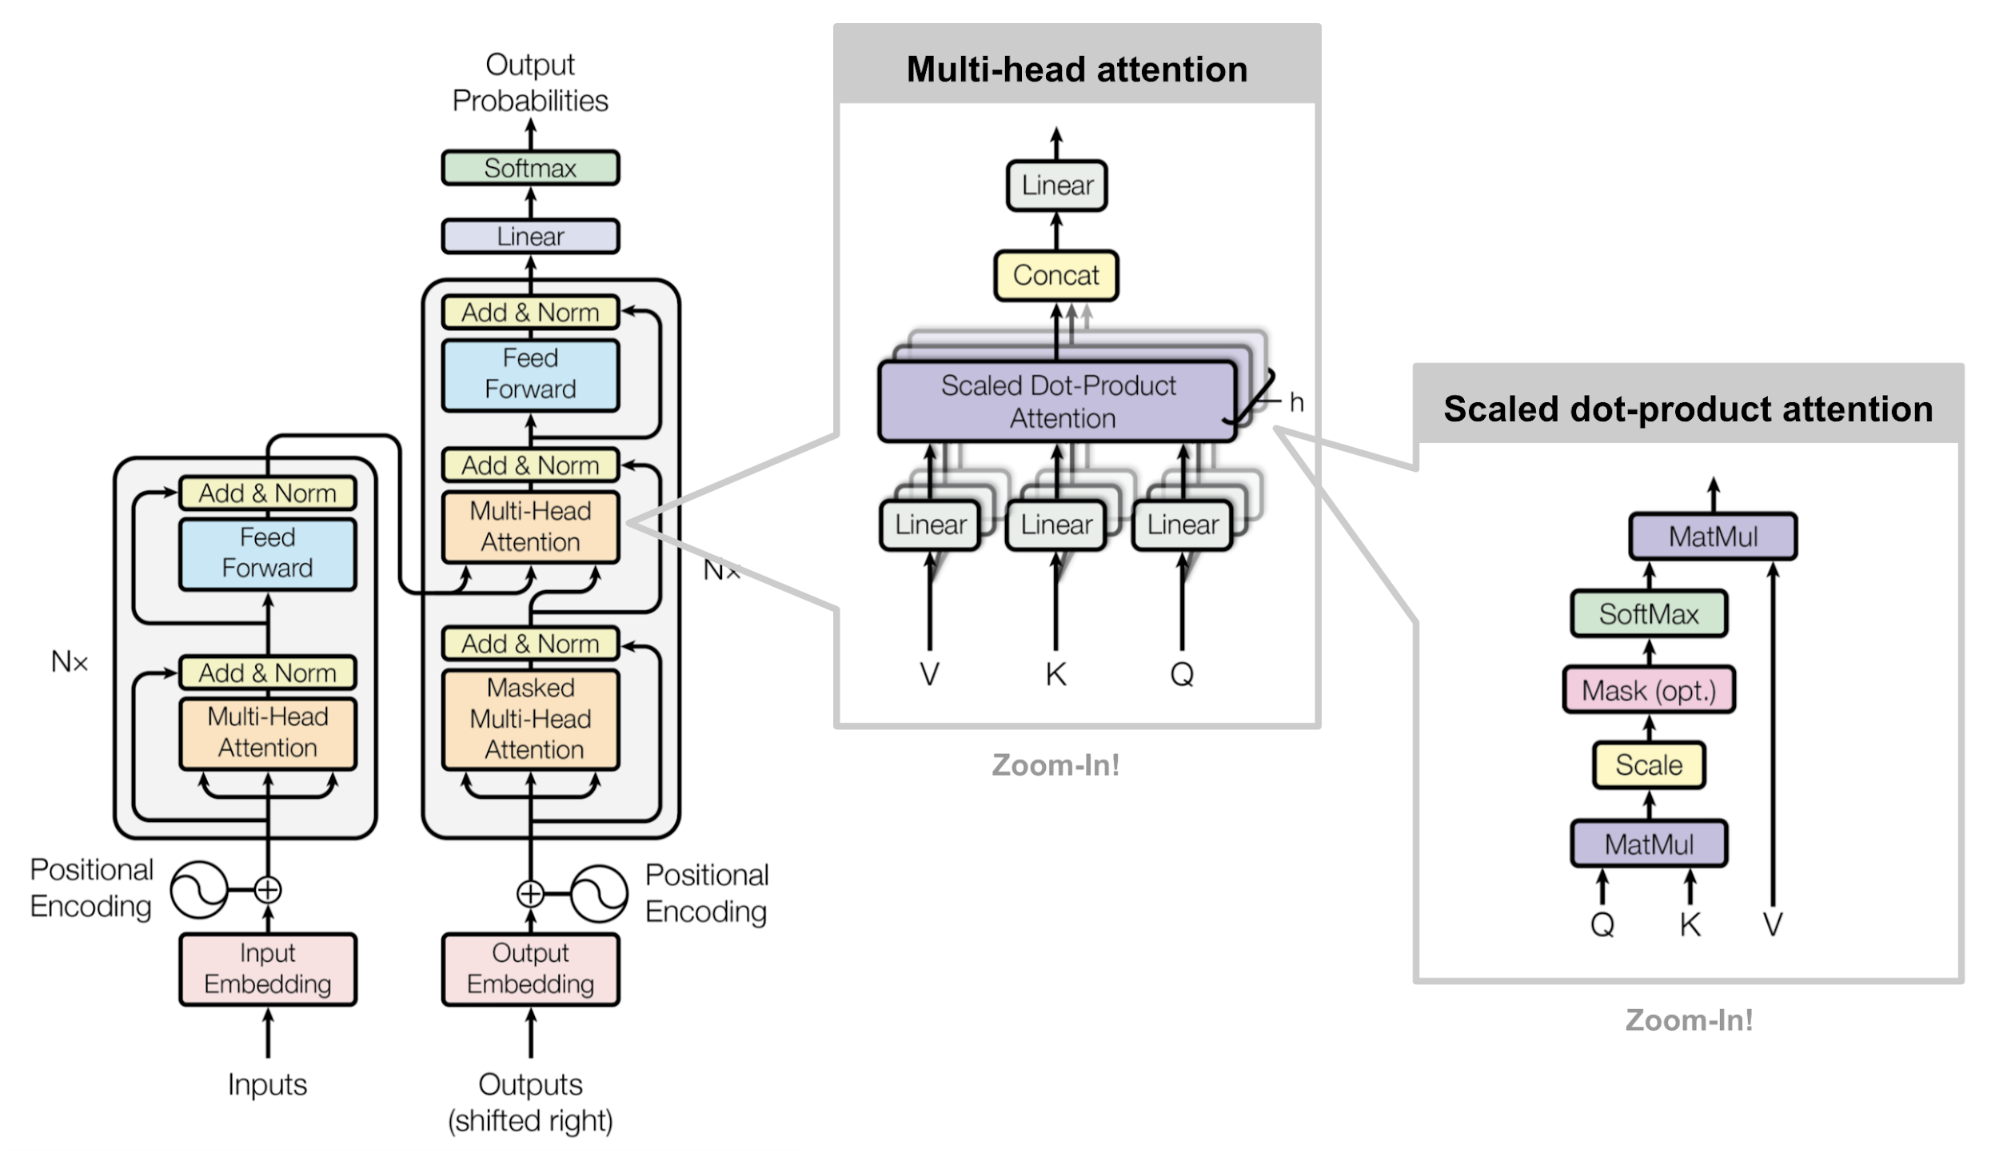
\includegraphics[width=0.8\textwidth]{transformer.png}
  \caption{Transformer architecture}
  \label{fig:transformer}
\end{figure}


\subsection{Vision Transformer}
\subsection{Swin Transformer}

